% Лабораторная работа по АСиСу № 2
% Михедов Константин Константинович

% Тип документа: статья, на бумаге А4
\documentclass[a4paper]{article}

% Подключение сторонних tex файлов 
\usepackage{import}


% Основные данные - ВУЗ, факультет, город...
\import{./../../stuff/tex}{config.tex}

% Подключение необходимых зависимостей
\import{./../../stuff/tex/settings}{packages.tex}
% Настройка подключенных пакетов
\import{./../../stuff/tex/settings}{preferences.tex}


% Шаблон титульной страницы 
\import{./../../stuff/tex/templates}{title.tex}
% Упрощенный блок "выполнил"
\import{./../../stuff/tex/templates}{sign1.tex}
% Макрос для содержания
\import{./../../stuff/tex/templates}{toc.tex}

% Определяем название документа
\title{
  Лабораторная работа №2 по курсу \\
  <<Компьютерный практикум <<Админимтрирование систем и сетей>>  
}
% Отключаем отображение правительства
\renewcommand{\government}{}
% Отключаем сокращенное нзавание университета
\renewcommand{\subuniversity}{}
% Указываем преподавателя
\renewcommand{\shortteachername}{Зудин Д.Е.}


% Путь до внешних изображений
\graphicspath{ {./figures/}}


% Основной текст работы
\begin{document}
  \templatedtitlepage
  
  \toc
  \section{Ход работы}

  \subsection{Захват пакетов}

  Для выполнения работы сначала необходимо определить, с помощью какого интерфейса выполняется
  доступ в Интернет и захватить 2-3 тысячи проходящих через него пакетов.
  
  Чтобы определиться с именем необходимого интерфейса воспользуемся утилитой \textit{nmcli}:
    
  \begin{figure}[H]
    \centering
    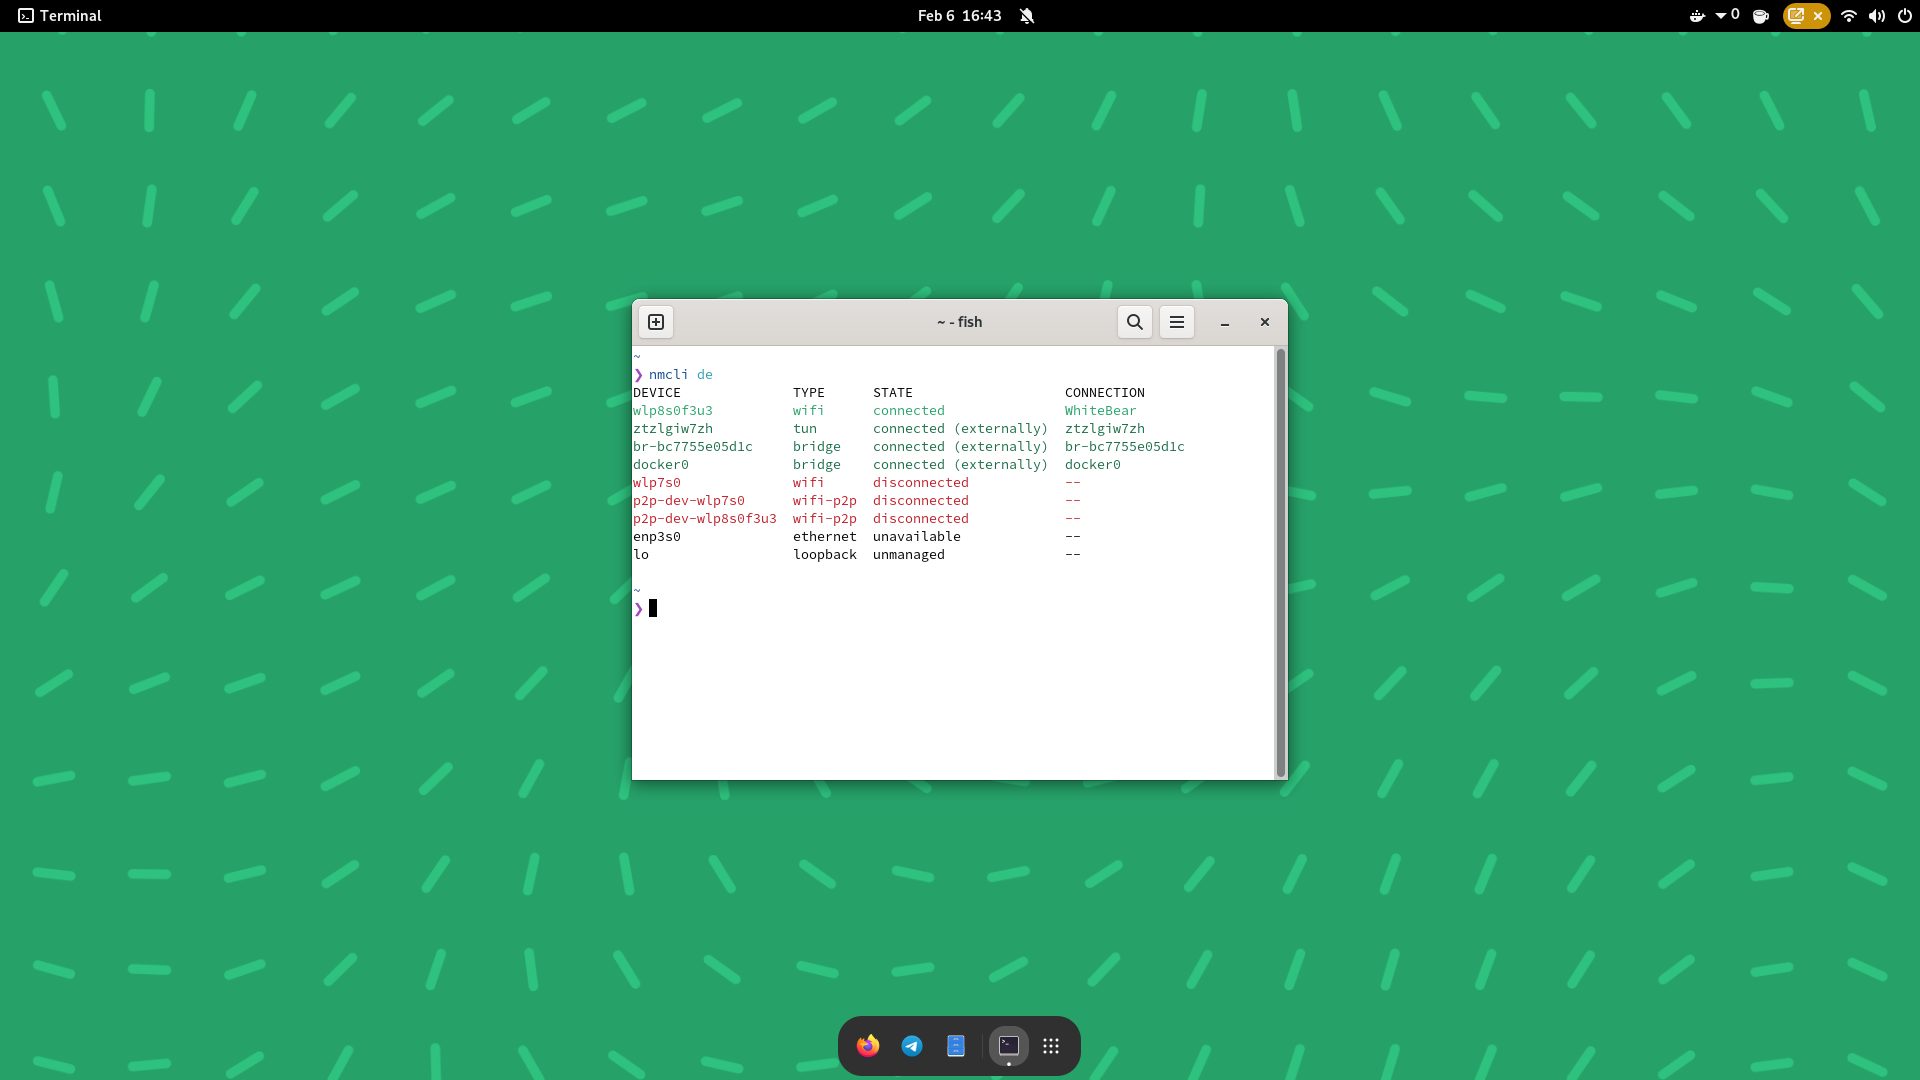
\includegraphics[width=1.0\textwidth]{02_0001}
    \caption{Информация о сетевых интерфейсах}
    \label{img:0001}
  \end{figure}

  Как видно из вывода программы (рис. \ref{img:0001} на стр. \pageref{img:0001}), для 
  доступа к Интернету используется интерфейс \textit{wlp8s0f3u3}, подключенный 
  к беспроводной сети с именем \textit{WhiteBear}.

  Получив имя необходимого интерфейса, запустим захват пакетов на нем при помощи
  \textit{Wireshark} (рис. \ref{img:0002} на стр. \pageref{img:0002}).

  \begin{figure}[H]
    \centering
    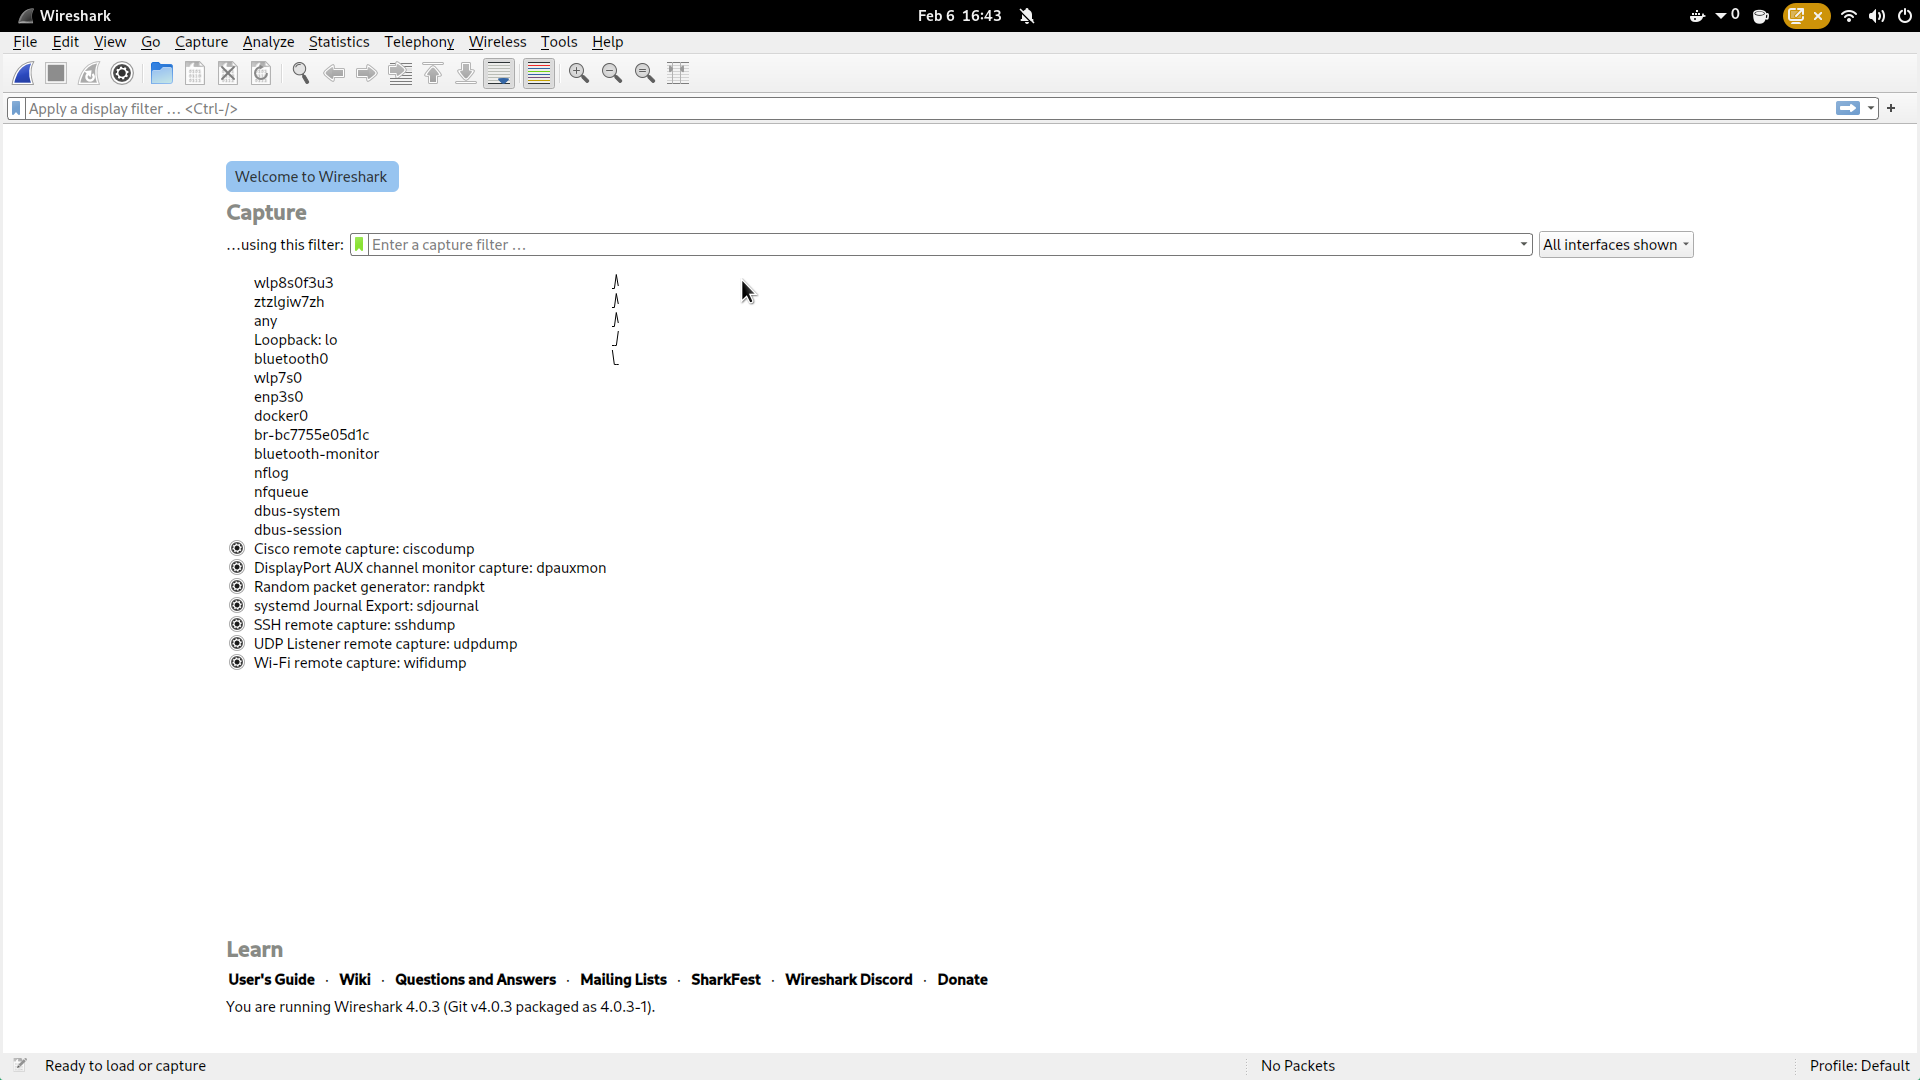
\includegraphics[width=0.9\textwidth]{02_0002}
    \caption{Запуск захвата пакетов}
    \label{img:0002}
  \end{figure}

  Для анализа потребуется захватить достаточно большое количество пакетов, поэтому,
  чтобы упростить и ускорить этот процесс, воспользуемся браузеров и перейдем на 
  страницу РУЗа (рис. \ref{img:0003} на стр. \pageref{img:0003}):
  
  \begin{figure}[H]
    \centering
    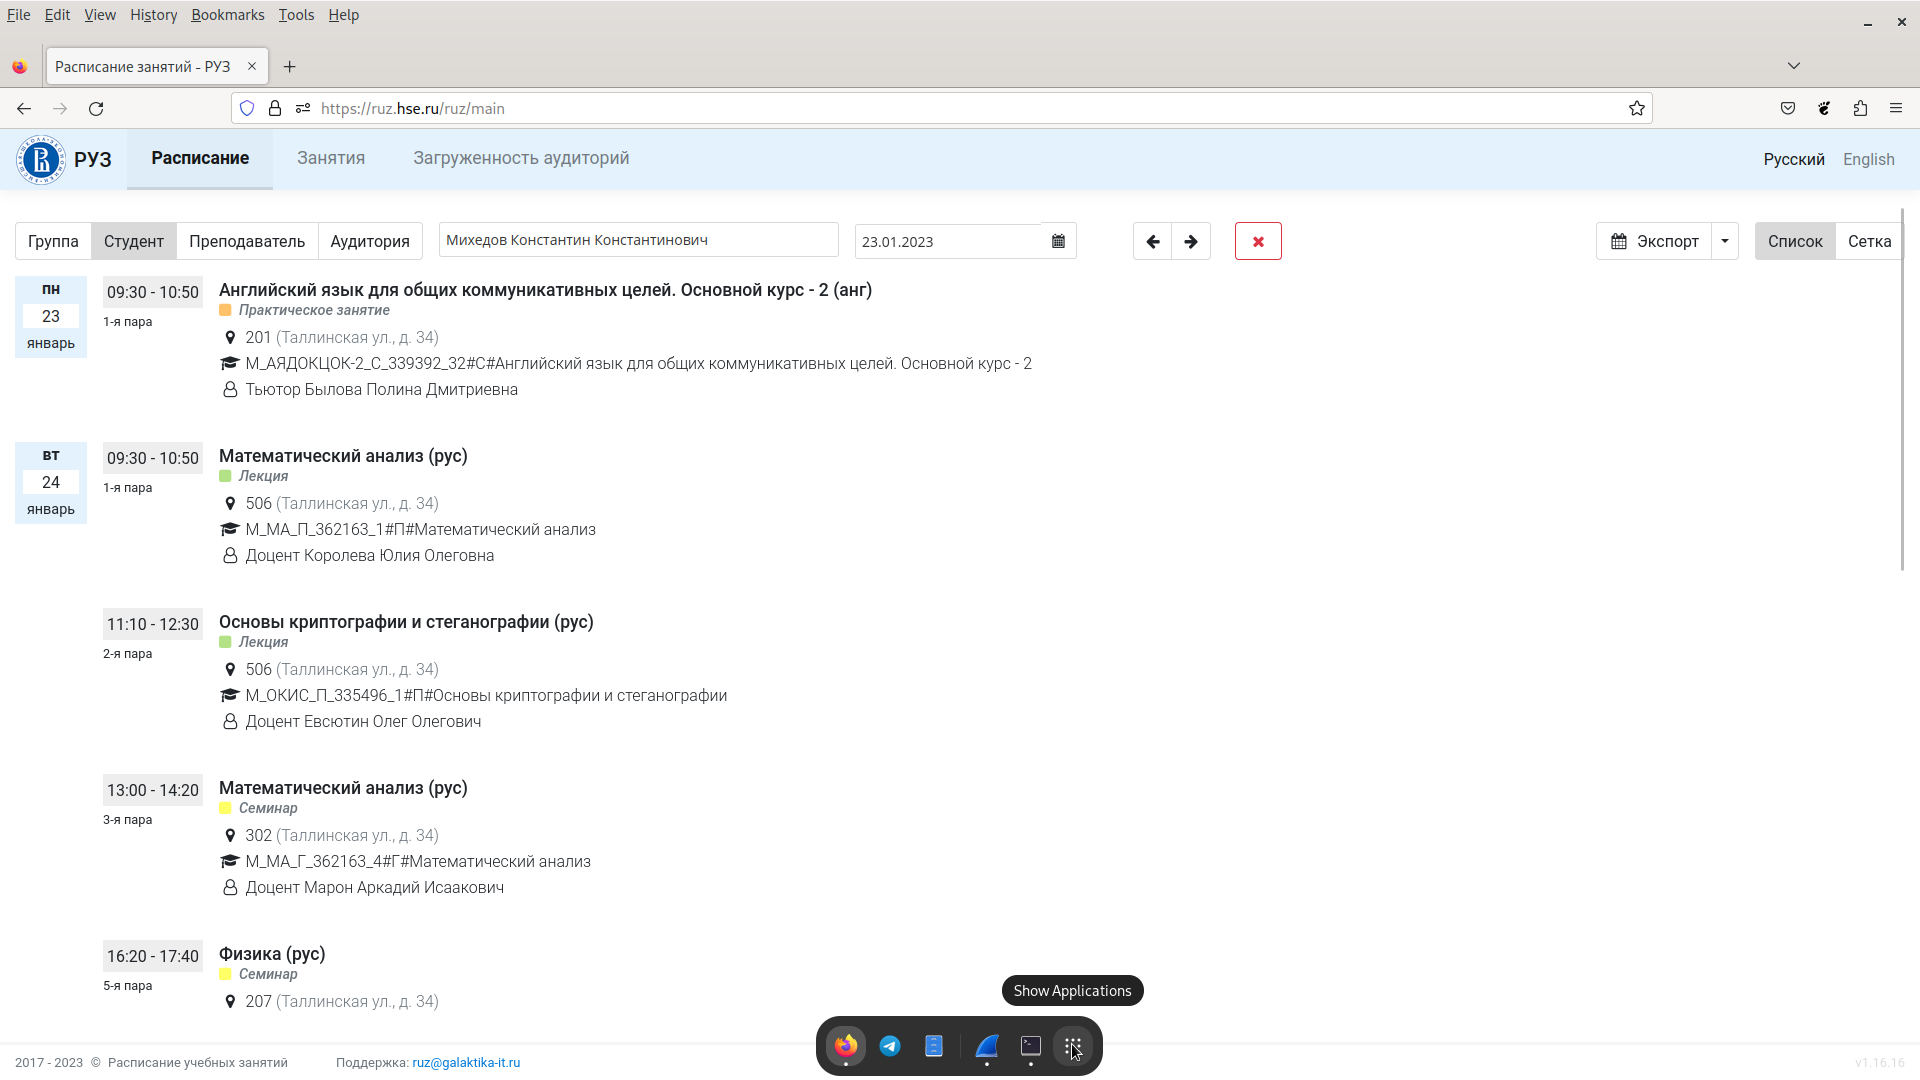
\includegraphics[width=0.9\textwidth]{02_0003}
    \caption{Ускоряем сбор пакетов просмотром web-страниц}
    \label{img:0003}
  \end{figure}

  Спустя некоторое время Интернет-серфинга наберется достаточное количество
  захваченный пакетов, тогда нужно будет остановить сниффинг, чтобы продолжить работу.

  \subsection{Фильтрация захваченных пакетов}

  \subsubsection{Отсеивание ICMP пакетов}

  Для того, чтобы отобразить только те пакеты, которые были переданны \textbf{не} по при помощи протокола 
  ICMP, воспользуемся встроенным в \textit{Wireshark} фильтром (рис. \ref{img:0005} на стр. \pageref{img:0005})

  \begin{figure}[H]
    \centering
    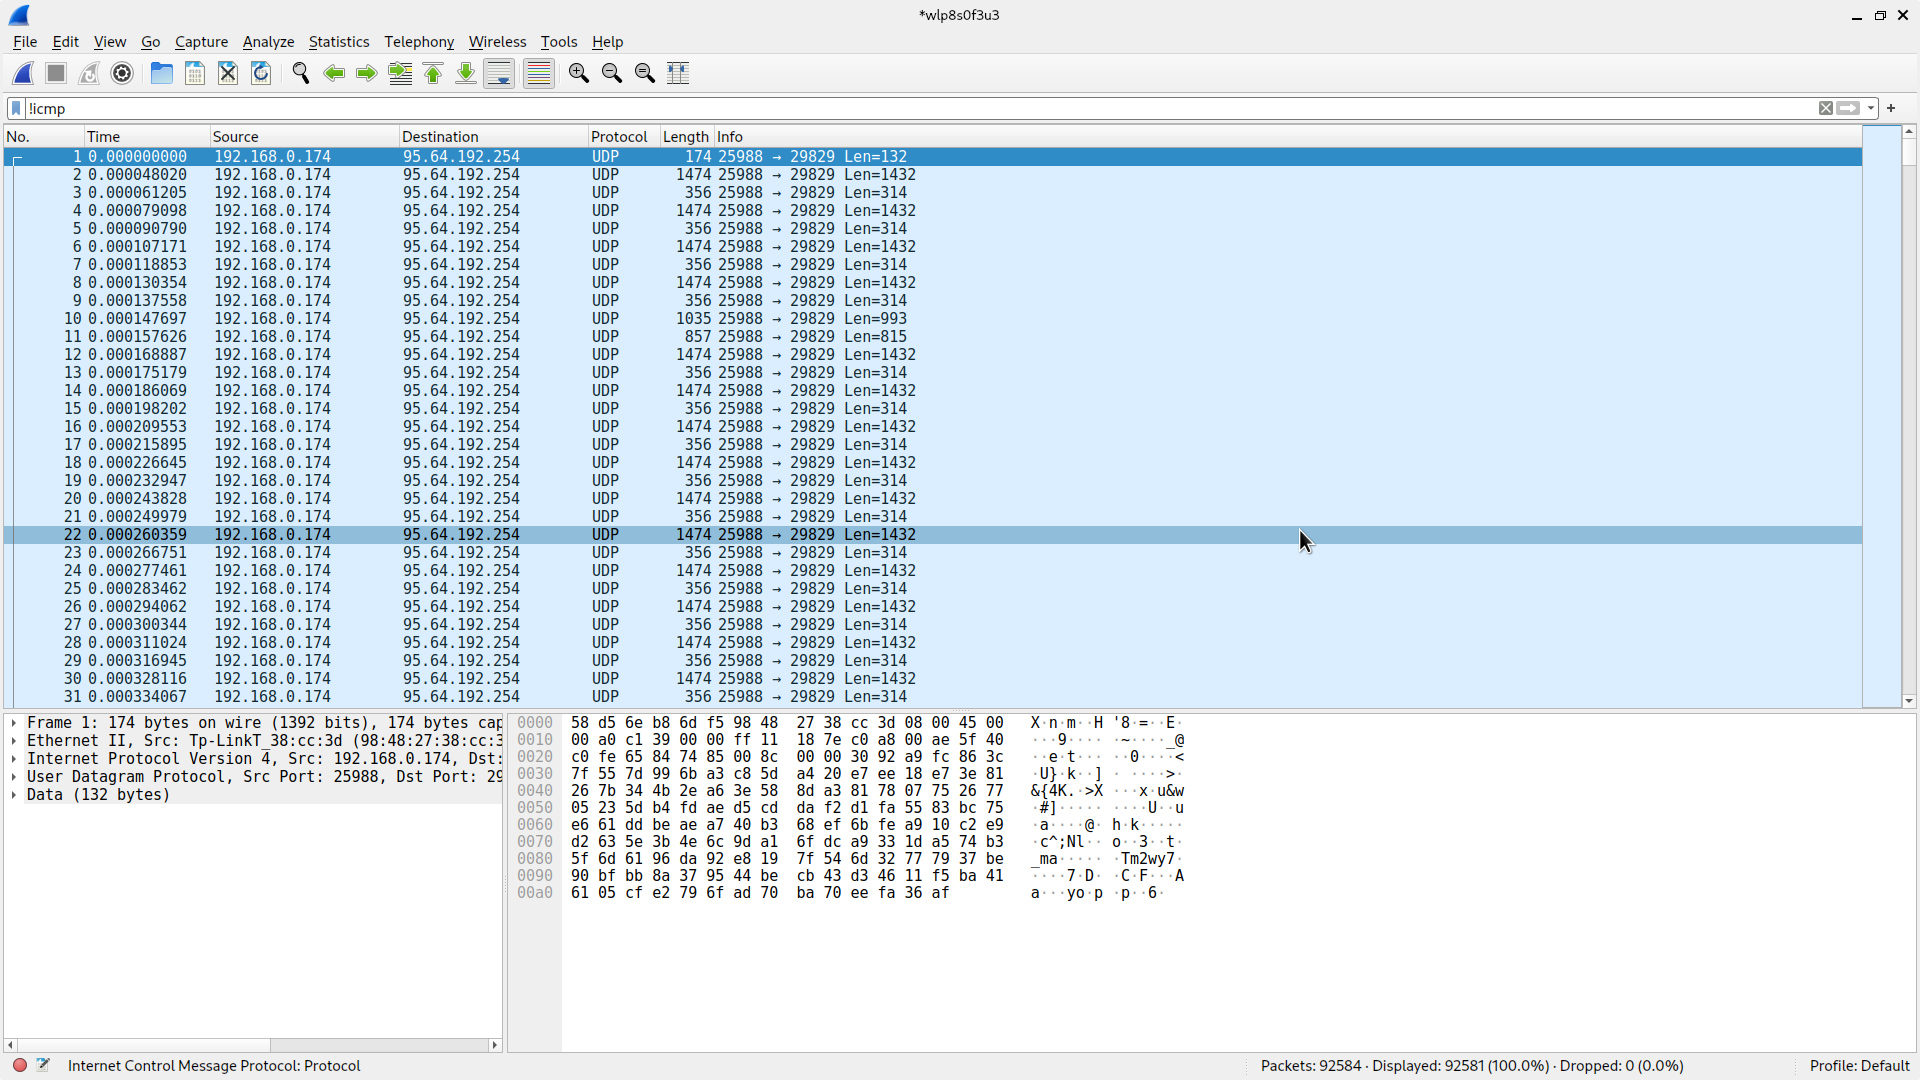
\includegraphics[width=0.9\textwidth]{02_0005}
    \caption{Убираем ICMP пакеты из выдачи при помощи фильтра \textit{!icmp}}
    \label{img:0005}
  \end{figure}

  Работа производилась на удаленной машине, подключение к которой выполнялось при помощи протокола RDP, поэтому 
  большинство захваченных пакетов являются пакетами, переданными протоколом UDP.
  Чтобы увидеть пакеты других типов (в частности HTTP пакеты, которые собирались 
  при помощи браузера) нужно отсеять еще и UDP пакеты (рис. \ref*{img:0006} на стр. \pageref{img:0006}).

  \begin{figure}[H]
    \centering
    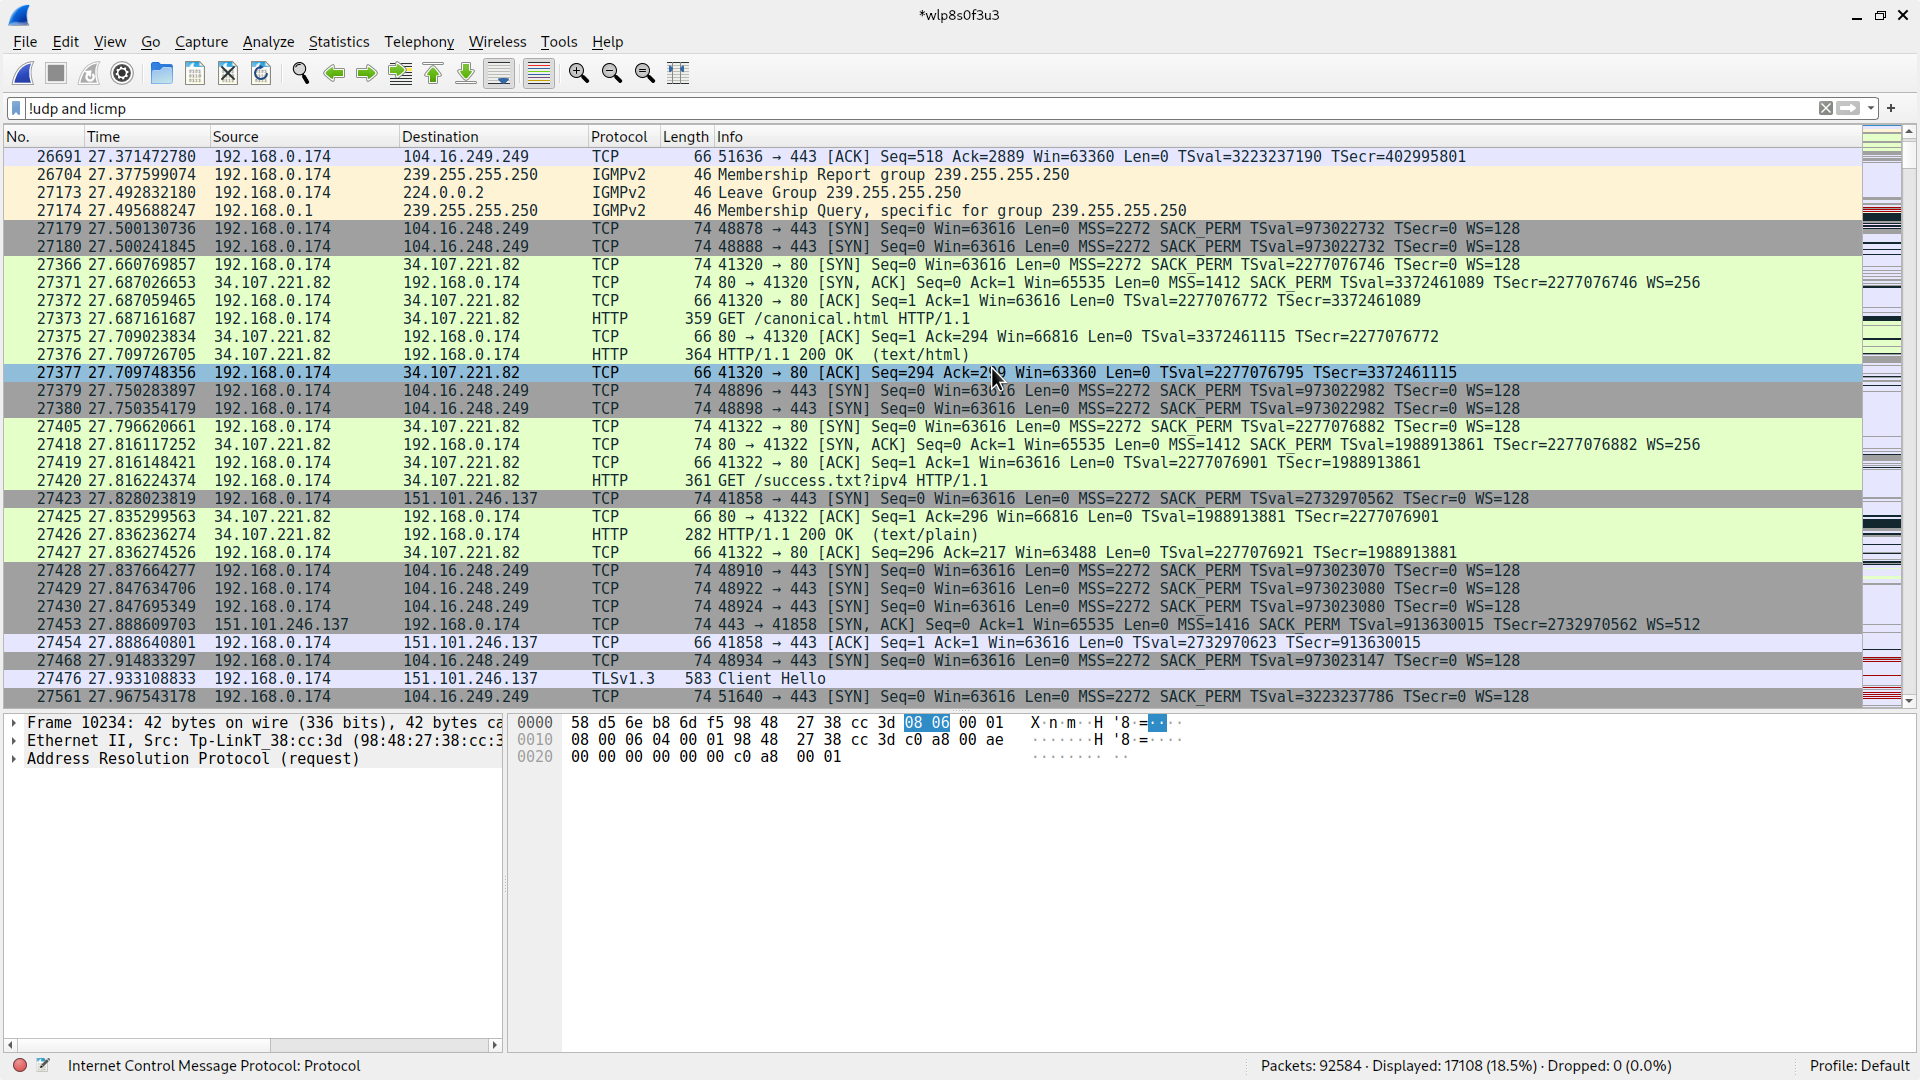
\includegraphics[width=0.9\textwidth]{02_0006}
    \caption{Отсеиваем UDP и ICMP пакеты фильтром \textit{!udp and !icmp}}
    \label{img:0006}
  \end{figure}

  \subsubsection{DNS и HTTP пакеты}

  Чтобы отобразить только те пакеты, которые были переданы при помощи или DNS,
  или HTTP, необходимо воспользоваться сложным условием и совместить
  два обычных фильтра при помощи дизъюнкции (рис. \ref{img:0007} на стр. \pageref{img:0007}) 
  
  \begin{figure}[H]
    \centering
    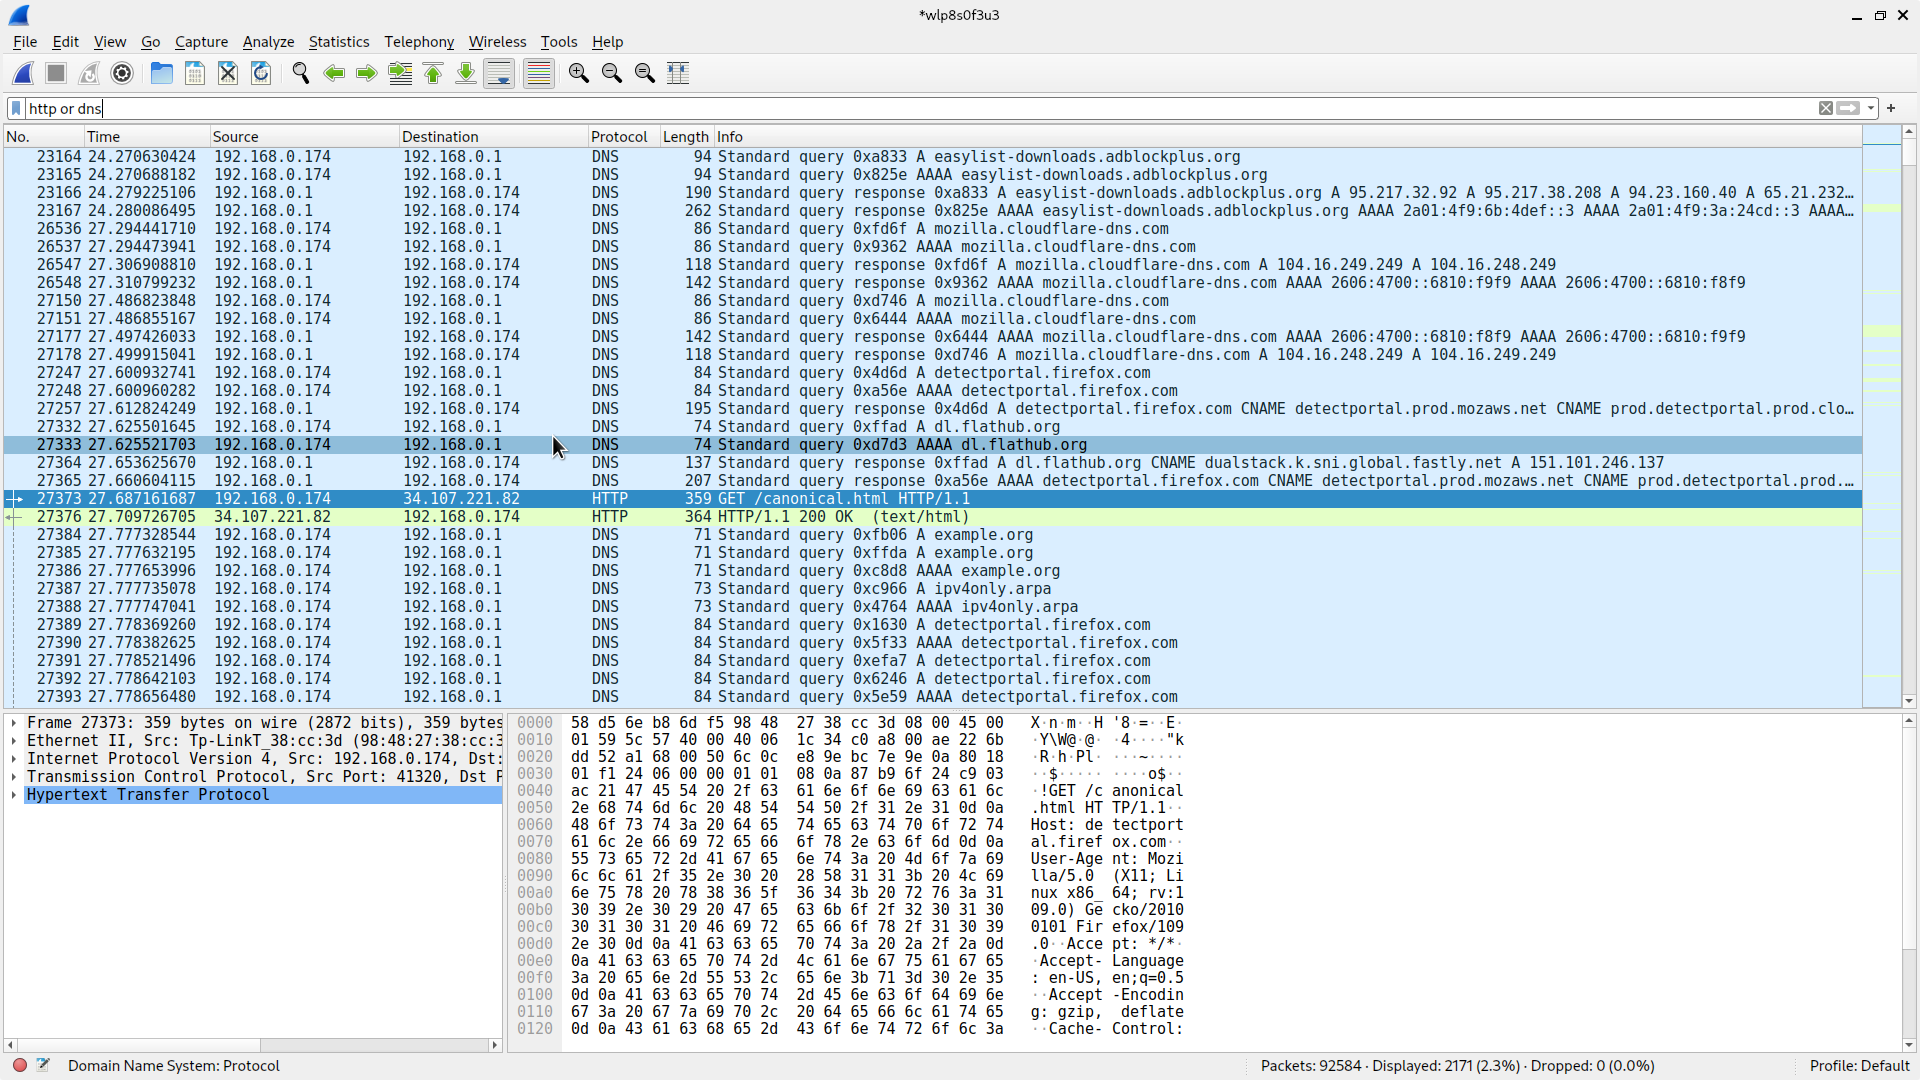
\includegraphics[width=0.9\textwidth]{02_0007}
    \caption{Отображаем только HTTP или DNS пакеты \textit{dns or http}}
    \label{img:0007}
  \end{figure}

  \subsubsection{Фильтрация по IP адресу}
  
  Для начала необходимо узнать IP адрес машины, на которой производился захват пакетов.
  Получить его можно при помощи утилиты \textit{ifconfig} и найденного ранее 
  имени интерфейса.

  \begin{figure}[H]
    \centering
    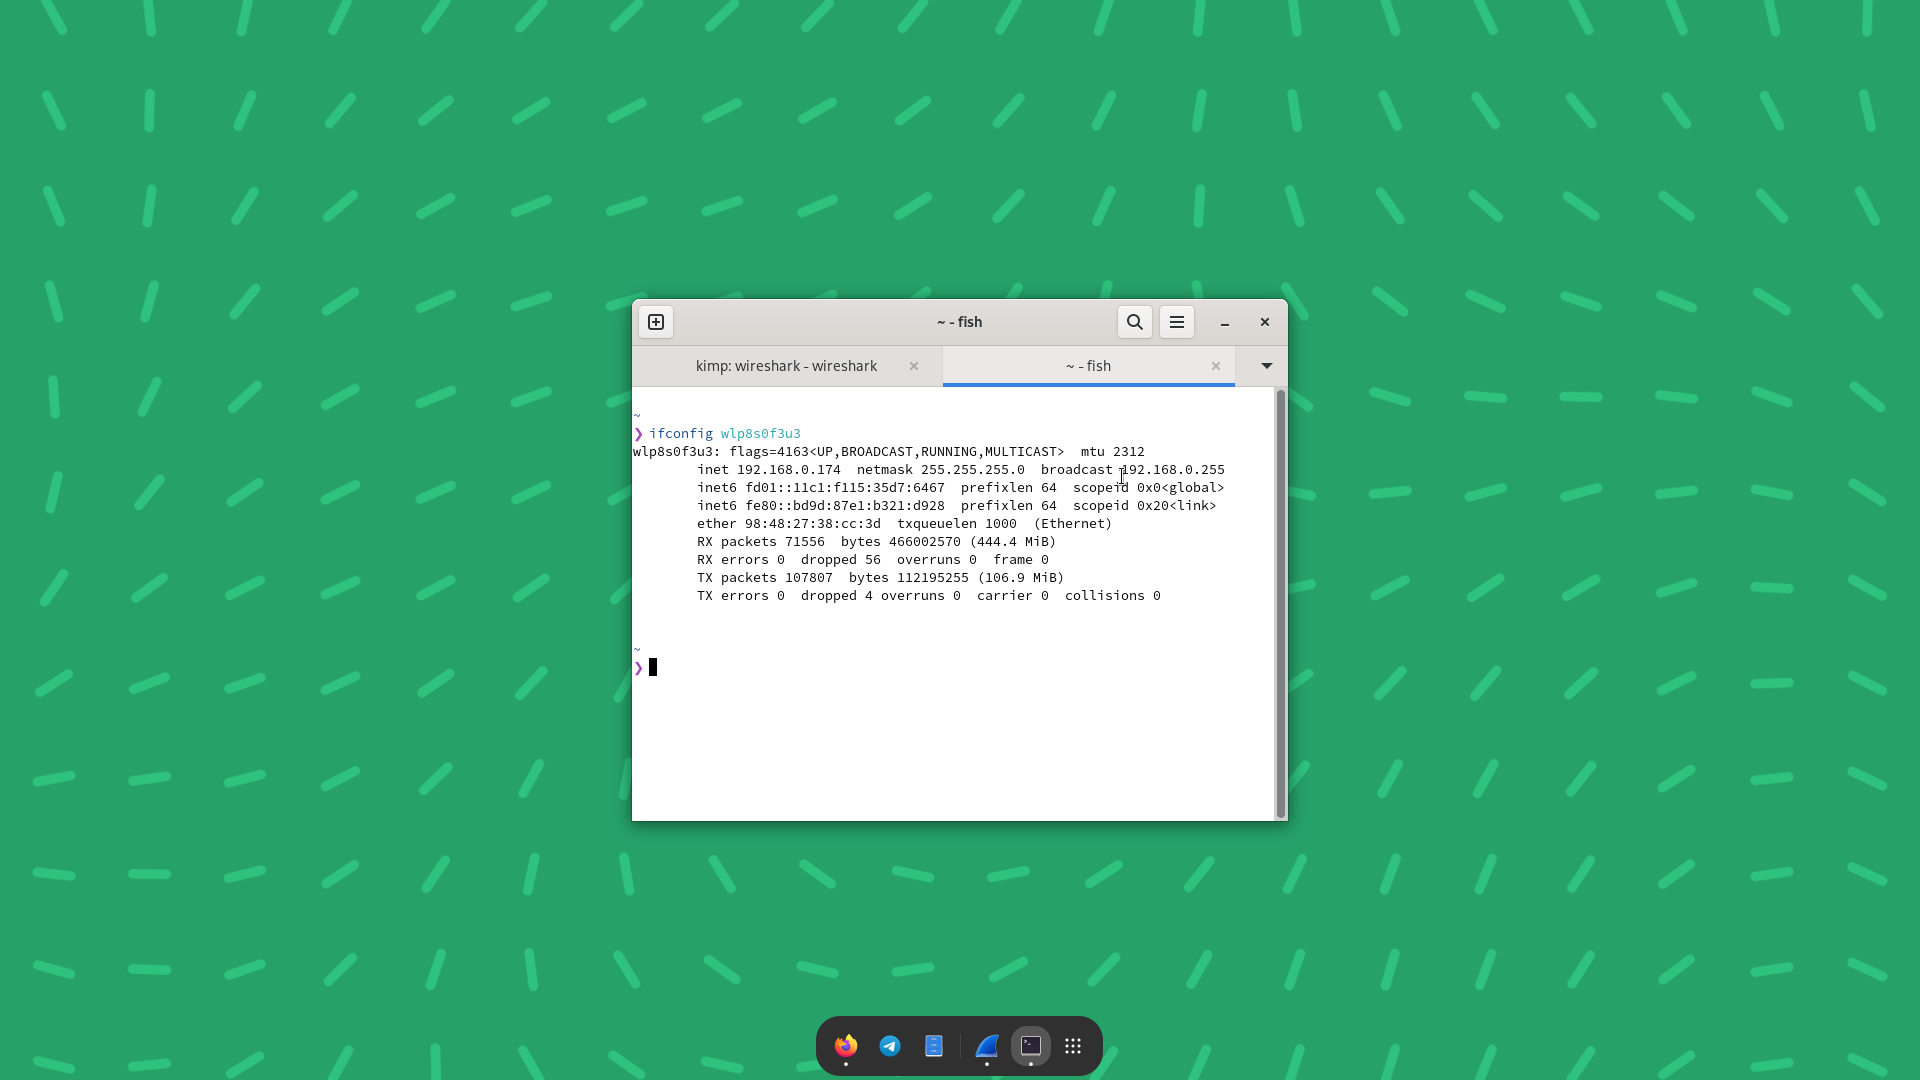
\includegraphics[width=0.9\textwidth]{02_0008}
    \caption{Получаем информацию о сетевом устройстве}
    \label{img:0008}
  \end{figure}

  Как видно из вывода программы - IPv4 адрес компьютера соответствует
  значению 192.168.0.174 (рис. \ref{img:0008} на стр. \pageref{img:0008}).

  Теперь отобразим только полученные извне пакеты (получатель - устройство с 
  IPv4 192.168.0.174) (рис. \ref{img:0009} на стр. \ref{img:0009}):

  \begin{figure}[H]
    \centering
    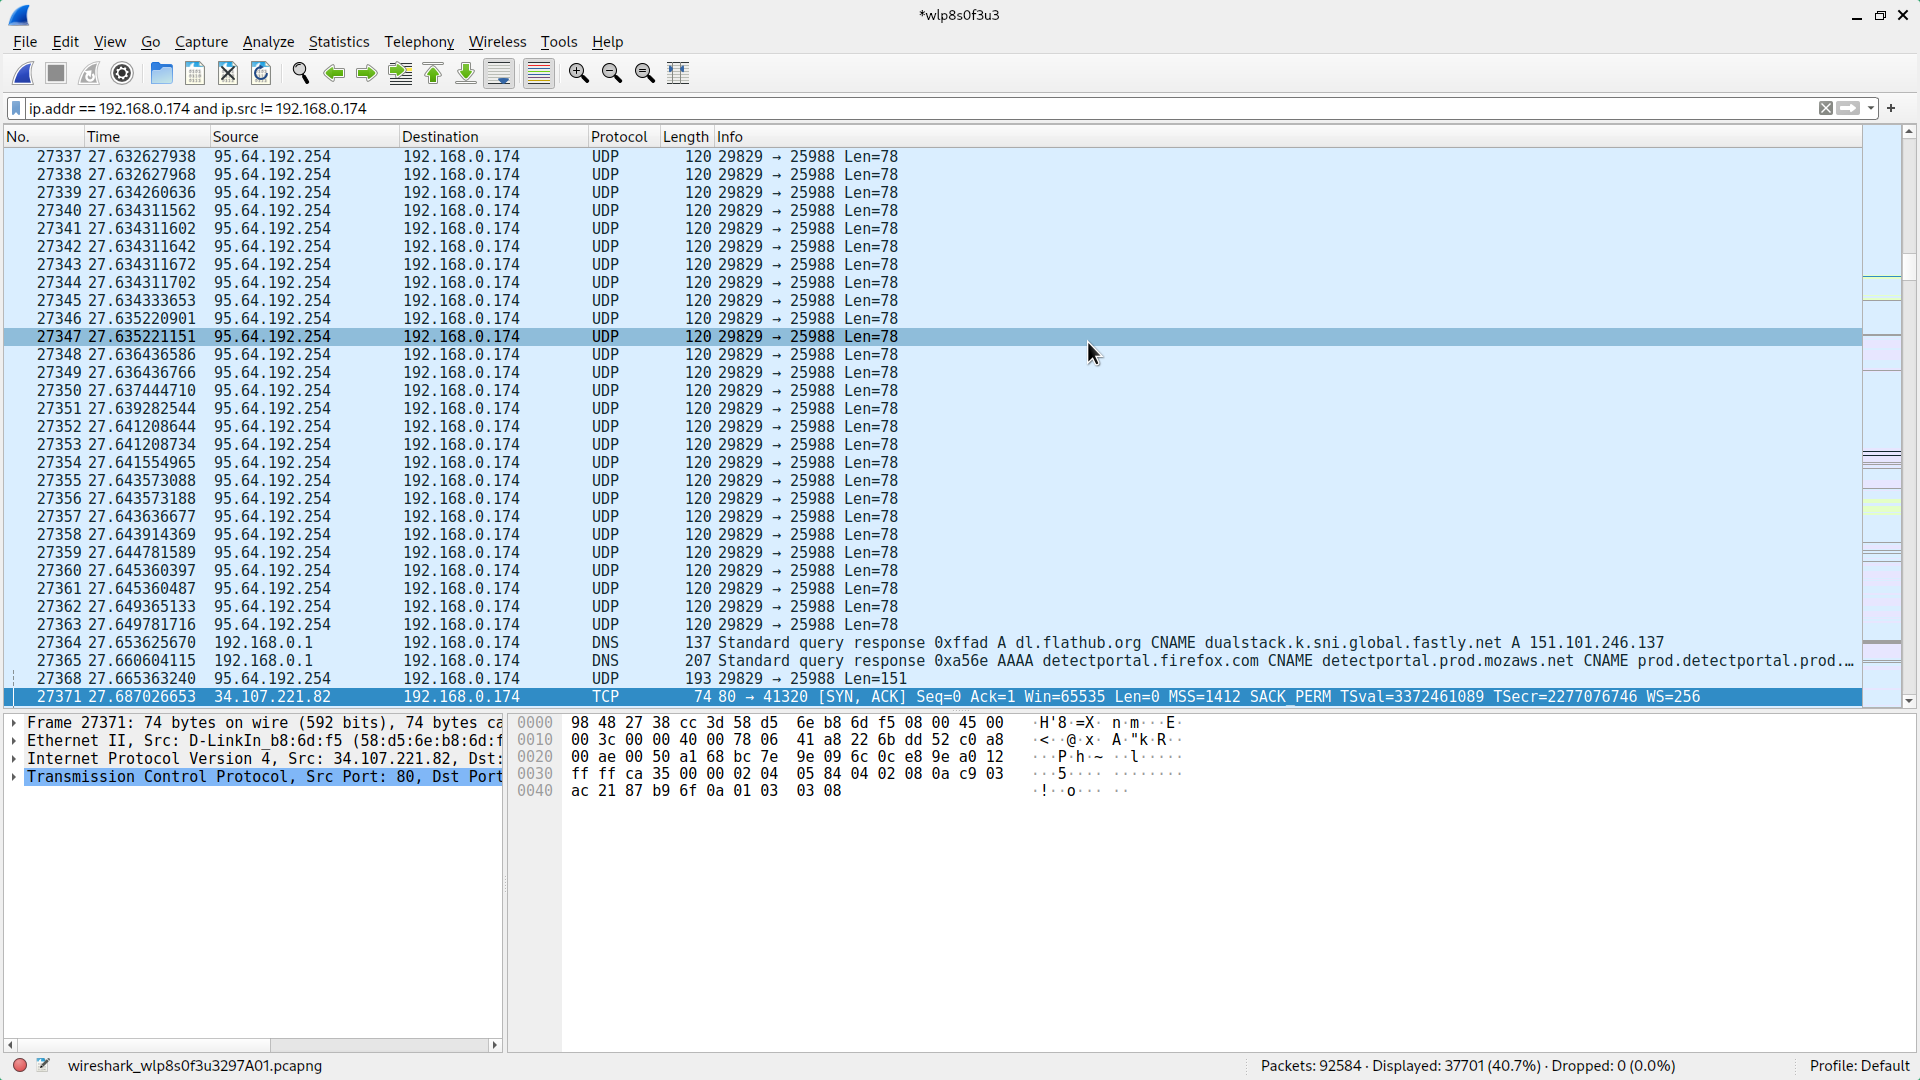
\includegraphics[width=0.8\textwidth]{02_0009}
    \caption{Просмотр полученный пакетов}
    \label{img:0009}
  \end{figure}

  В данном случае используется сложное условие вида
  \textit{ip.addr = ... and ip.src != ...}, которое дословно означает:
  отобразить пакеты, в которых в качестве или отправителя содержится определенный
  IPv4 адре и в которых при этом этот адрес не является адресом отправителя.
  Можно было сделать тоже самое проще: \textit{ip.dst = ...}.

  \subsubsection{IPv6 пакеты}

  Чтобы отобразить пакеты, отправленные или полученные при помощи IPv6 воспользуемся фильтром 
  \textit{ip.version == 6} (рис. \ref{img:0010} на стр. \pageref{img:0010}).

  \begin{figure}[H]
    \centering
    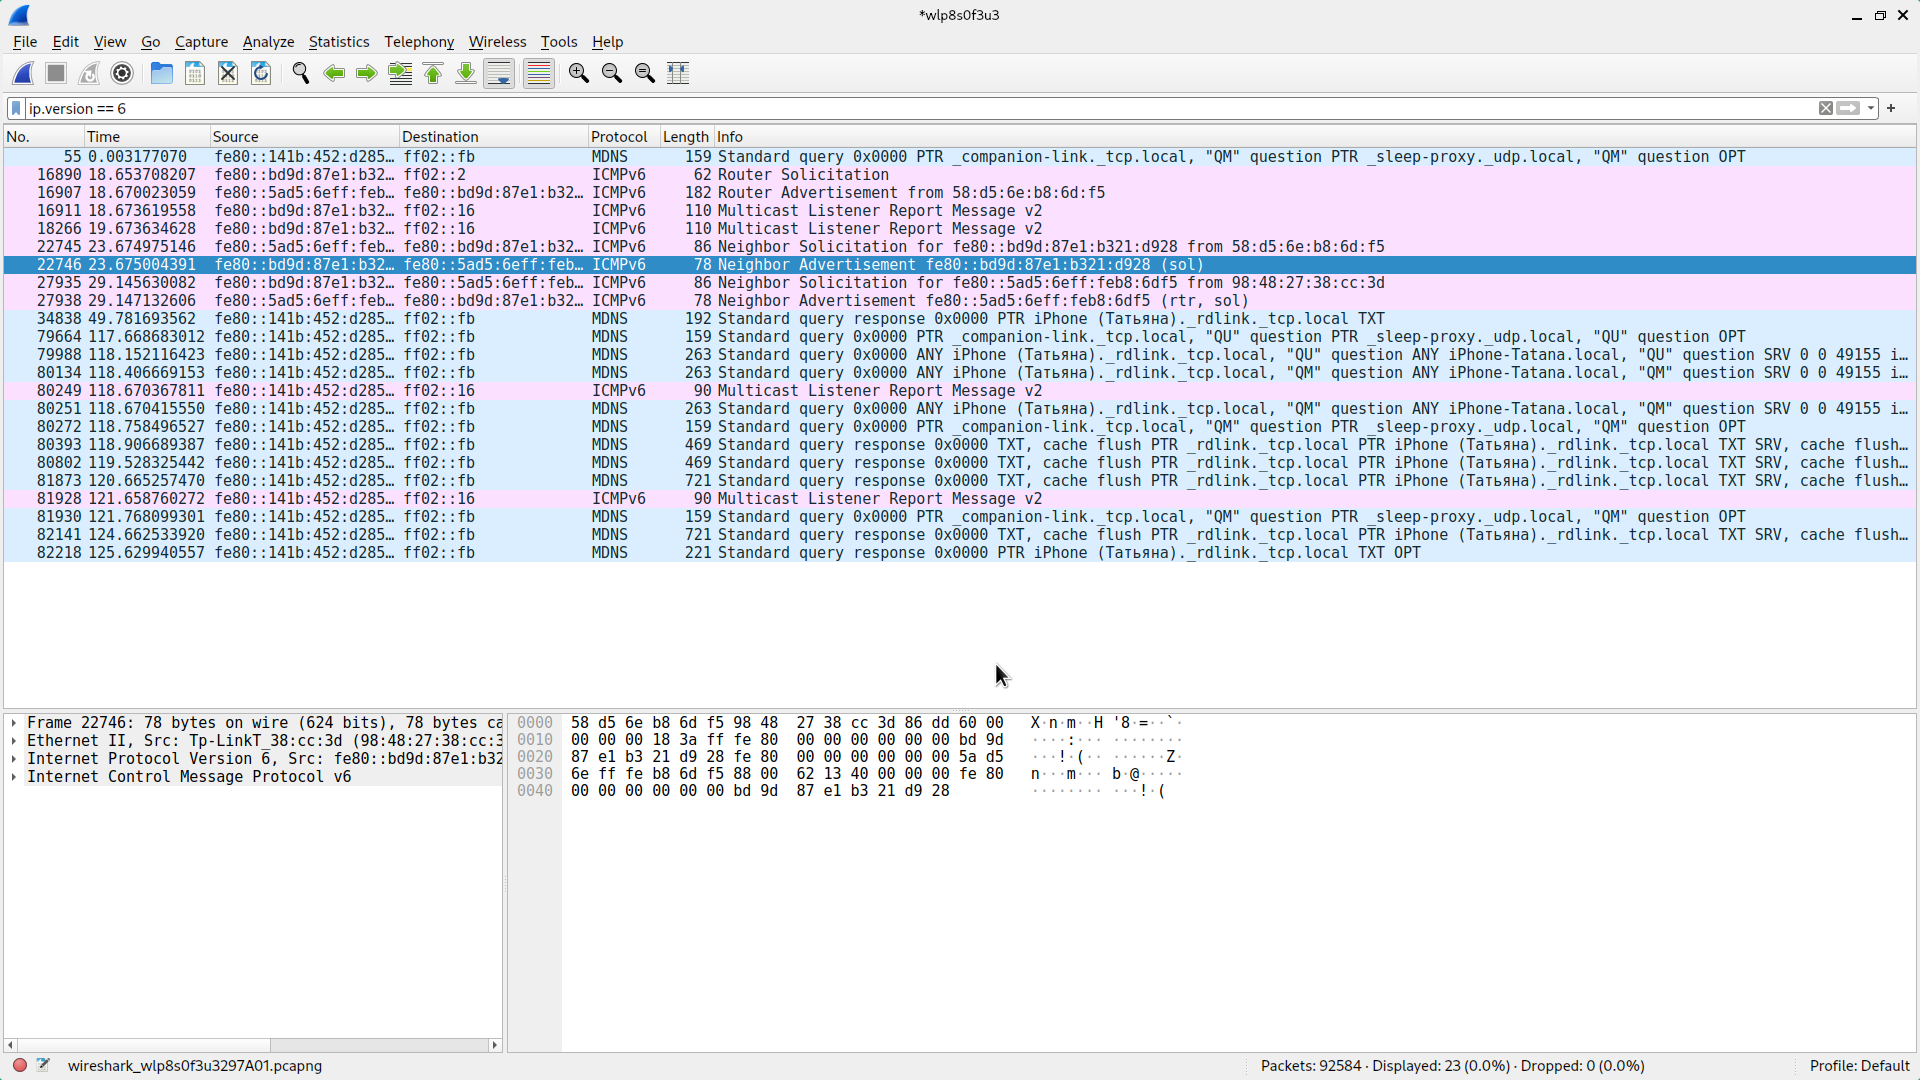
\includegraphics[width=0.8\textwidth]{02_0010}
    \caption{Пакеты, отправленные при помощи IPv6}
    \label{img:0010}
  \end{figure}

  Такого же ответа можно добиться и при помощи другого фильтра, например \textit{ipv6.dst != ipv6.src}

  \subsection{Анализ при помощи графического представления}

  \textit{Wireshark} предоставляет огромнные возможности для статичстического анализа трафика
  и перехваченный пакетов. Так, есть возможность посмотреть график нагрузки на сеть, для того,
  чтобы его увидеть, откроем меню \textit{Statistics} и выберем опцию \textit{I/O Graphs}
  (рис. \ref{img:0011} на стр. \pageref{img:0011}):

  \begin{figure}[H]
    \centering
    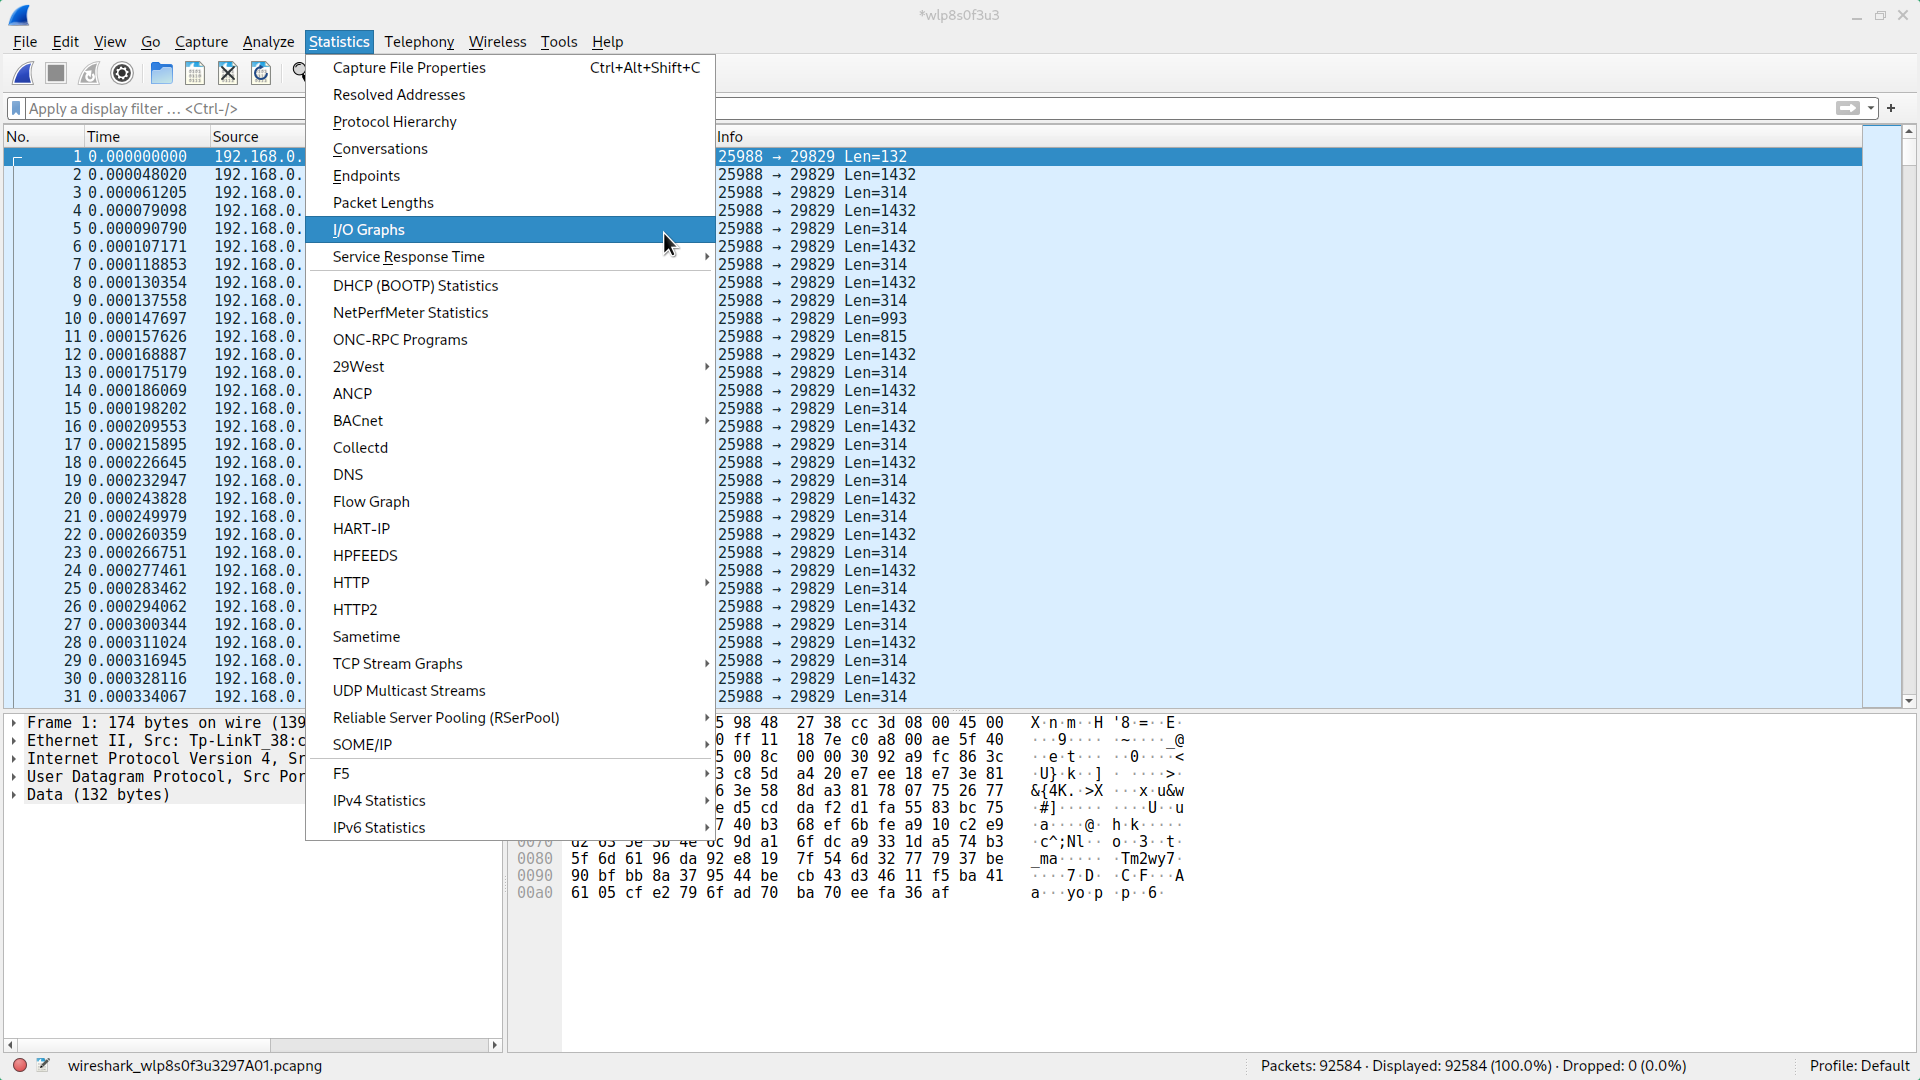
\includegraphics[width=0.9\textwidth]{02_0011}
    \caption{Открываем график для анализа}
    \label{img:0011}
  \end{figure}

  По умолчанию на графике будут отображены количество пакетов, захваченных за один момент
  времени (черная кривая) и количество ошибок TCP-соединений (красная гистограмма)
  как на рис. \ref{img:0012} на стр. \pageref{img:0012}.

  \begin{figure}[H]
    \centering
    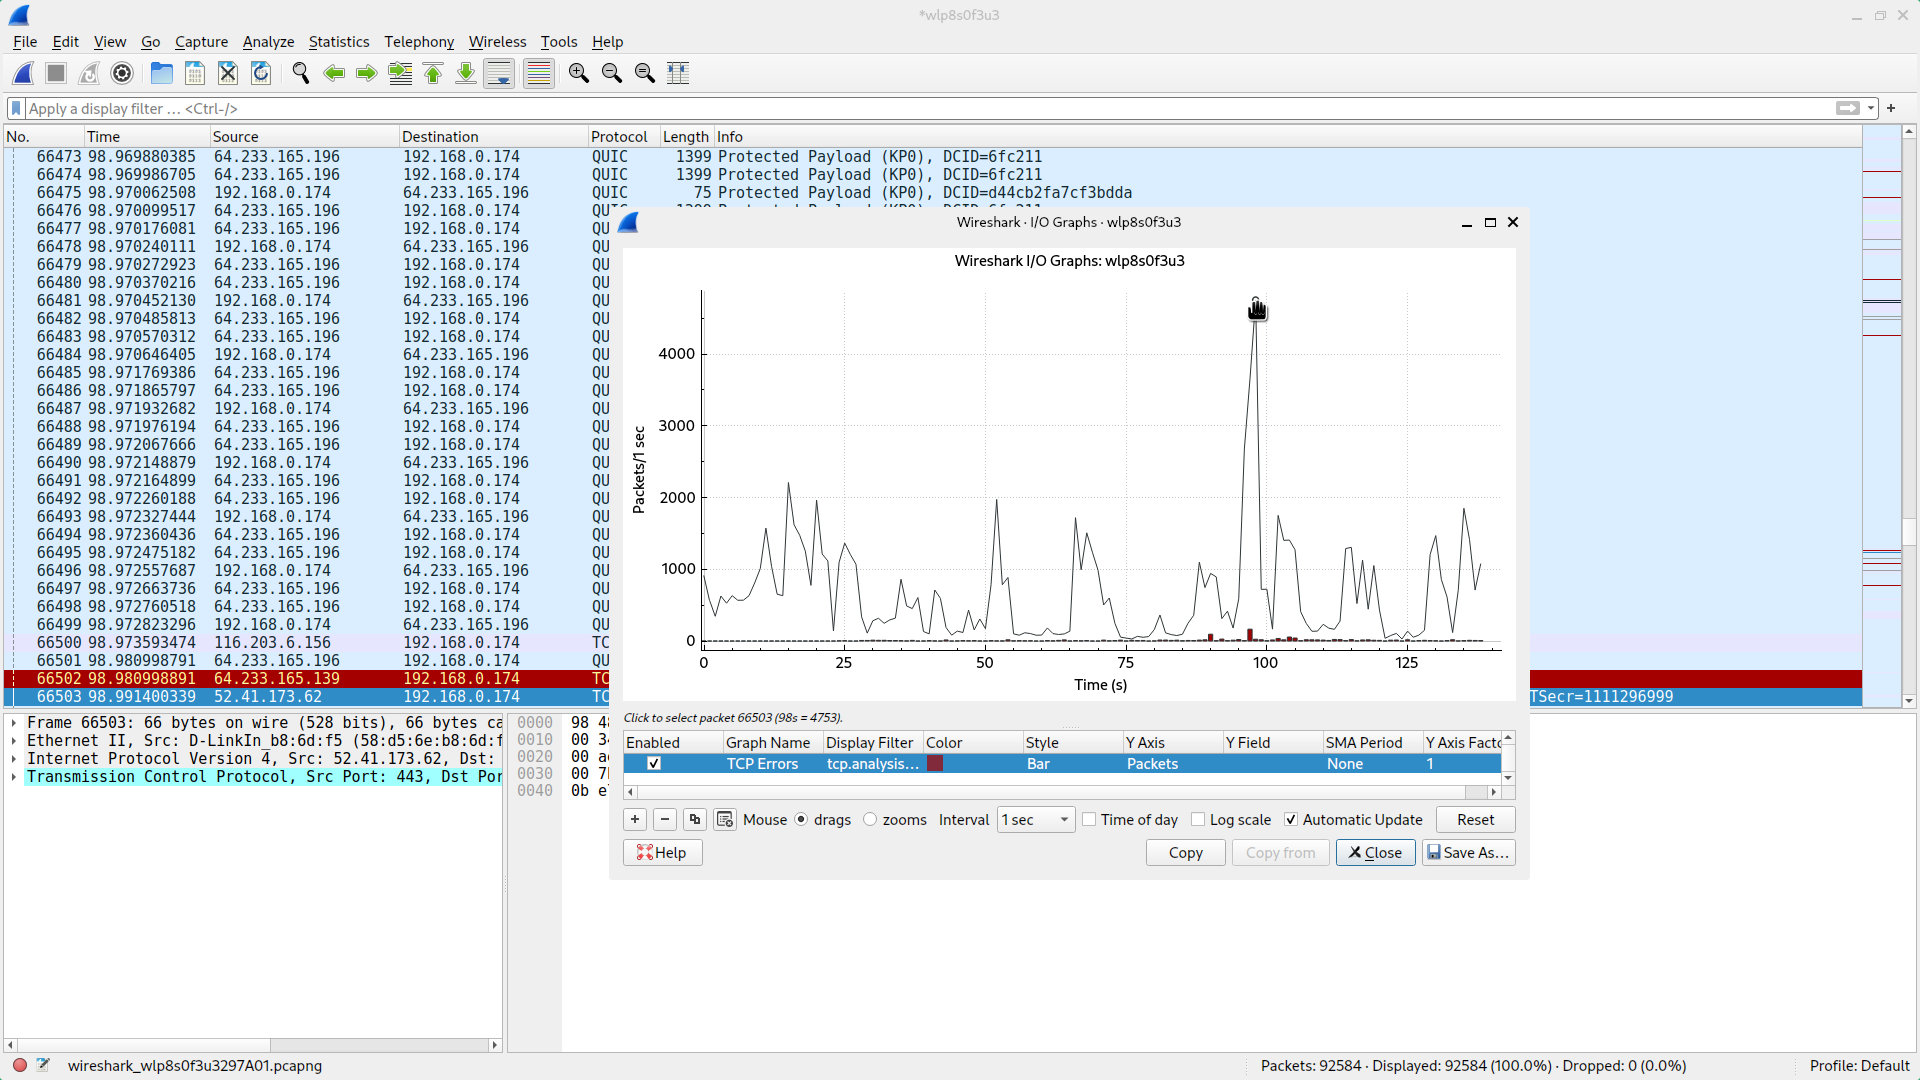
\includegraphics[width=1.0\textwidth]{02_0012}
    \caption{График со статистическими показателями}
    \label{img:0012}
  \end{figure}

  По данному графику видно, что наибольшая нагрузка на сеть происходила с 95-ой по 
  100-ую секунду захвата пакетов, в том же интервале наблюдалось максимальное количество
  ошибок в TCP-соединениях. Пиковая нагрузка на сеть составляет почти 5000 пакетов в секунду,
  а так как скорость захвата пакетов растет вместе с их количеством, можно сделать вывод,
  что в момент пиковой нагрузки скорость захвата выросла примерно на 4500 пакетов в секунду.

  На графическое представление также можно накладываь различные фильтры, например посмотреть 
  статистику только по перехваченным HTTP пакетам (рис. \ref{img:0013} на стр. \pageref{img:0013})

  \begin{figure}[H]
    \centering
    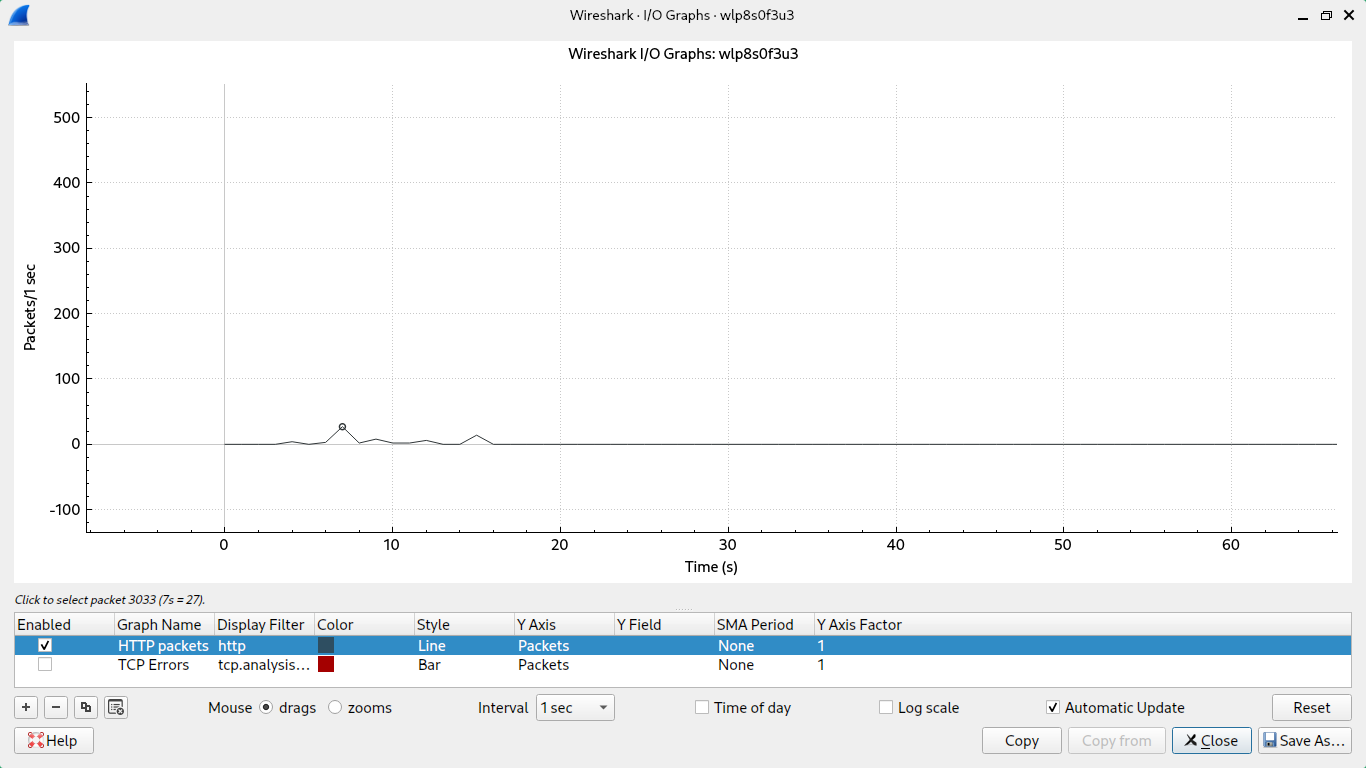
\includegraphics[width=1.0\textwidth]{02_0013}
    \caption{Статистика по перехваченным HTTP пакетам}
    \label{img:0013}
  \end{figure}

  \section{Вывод}

  В ходе данной лабораторной работы мне удалось разобраться со встроенным в 
  \textit{Wireshark} фильтром пакетов, попрактиковаться в составление сложных 
  условий а также проанализировать статистические показатели сети при помощи их 
  графического представления.
\end{document}
